\documentclass[final,5p,times,number,sort&compress]{elsarticle}

\usepackage{amsmath,amssymb}
\usepackage{booktabs}
\usepackage{graphicx}
\usepackage{multirow}
\usepackage{array}
\usepackage{microtype}
\usepackage{url}
\usepackage{hyperref}
\hypersetup{hidelinks}
\usepackage{enumitem}
\emergencystretch=1.5em

\journal{Future Generation Computer Systems}

\newcommand{\systemname}{Semantic Layer Workflow}
\newcommand{\imageDOM}{Image DOM}
\newcommand{\vect}[1]{\boldsymbol{#1}}
\newcommand{\mask}{\mathbf{M}}
\newcommand{\loss}{\mathcal{L}}
\newcommand{\policy}{\pi}

\begin{document}

\begin{frontmatter}

\title{Semantic Layer Workflows for Adaptive Generative AI Editing in the Compute Continuum}

\author[inst1]{Stelios Sotiriadis\corref{cor1}}
\ead{s.sotiriadis@bbk.ac.uk}
\cortext[cor1]{Corresponding author.}
\address[inst1]{School of Computing and Mathematical Sciences, Birkbeck, University of London, London, United Kingdom}

\begin{abstract}
Interactive diffusion editing is usually a session, not a single model call. A user generates an image, selects a region, tries alternatives, preserves surrounding content, and may roll back. Full-image regeneration repeats work and often changes non-target regions, while one-off inpainting does not provide reusable semantic state, provenance, or scheduling information.

This paper introduces \systemname{}, a workflow model that represents an image as a graph of semantic layers with masks, bounding boxes, labels, edit history, provenance, cache keys, and execution metadata. The workflow chooses among full regeneration, semantic local diffusion, cached re-editing, deterministic projection, and rollback according to edit scope, latency, preservation risk, and available layer state. The aim is not to replace diffusion editing models, but to make iterative editing schedulable and reproducible across heterogeneous compute resources.

The prototype combines Stable Diffusion and SDXL pipelines with GroundingDINO+SAM2 annotation, crop-local diffusion, mask compositing, projection-only color edits, and persisted versions. The evaluation covers 200 paired local executions across 10 checkpoints, four edit categories, and five seeds, plus measured NVIDIA L4 and T4 tiers. On Apple MPS, semantic rendering is 1.788x faster than full regeneration without detector cost, but detector-inclusive first edits average 0.809x because annotation costs 13.543 s. Cached re-edits reach 7.041x speedup. On an NVIDIA L4, detector-inclusive first edits average 4.28x speedup; seven long edit sessions across five model families reduce 303 full-regeneration variants from 2786.7 s to 528.9 s, giving 5.37x mean speedup while preserving non-target pixels under the implemented compositing metrics.
\end{abstract}

\begin{keyword}
Compute continuum \sep Scientific workflows \sep Generative AI \sep Diffusion models \sep Semantic layers \sep Provenance \sep Adaptive execution \sep Workflow scheduling \sep Reproducibility \sep Performance modeling
\end{keyword}

\end{frontmatter}

\section{Introduction}

Generative AI pipelines are becoming data- and compute-intensive workflows. In interactive image editing, users iterate: generate an image, identify a region, alter an object or color, undo a variant, preserve identity, and compare alternatives. Each iteration may require detector inference, segmentation, denoising, compositing, metric evaluation, and provenance updates. The process therefore has core properties of scientific workflow execution: heterogeneous tasks, data dependencies, intermediate artifacts, repeated execution, and trade-offs between latency, quality, and resource cost \citep{deelman2009workflows,liew2017scientific,ferreiradasilva2017characterization}.

Current diffusion editors synthesize well but manage workflow state poorly. Full-image regeneration recomputes everything and often changes unrelated pixels. Manual inpainting gives local control, but depends on user effort and lacks reusable semantic state. Prompt editing, cross-attention control, ControlNet, and instruction-tuned editors improve controllability \citep{hertz2023prompt,zhang2023controlnet,brooks2023instructpix2pix}, but most pipelines still lack named regions, edit histories, cached masks, rollback states, and policy-driven execution.

This paper represents iterative diffusion editing as a semantic scientific workflow. The image is an \imageDOM{}: a graph of named semantic layers with provenance, dependency context, and cached execution state. An edit request becomes a workflow decision. Simple color updates may use deterministic projection; texture changes may use semantic local diffusion; global or entangled edits may require full regeneration; repeated edits and rollback can reuse stored layer state.

This framing matters for compute-continuum systems because the workflow exposes information hidden by monolithic generation calls: region size, expected cost, cache availability, dependency risk, provenance constraints, and candidate operators. The evaluation combines a local benchmark, measured GCP L4 and T4 tiers, and resource-sensitivity projections; it is not yet a deployed edge-cloud-HPC scheduler.

We make four contributions.

\begin{enumerate}[leftmargin=*]
    \item We define a semantic layer workflow model for diffusion editing, including layer graphs, edit operators, provenance records, cache keys, and version states.
    \item We formulate adaptive editing as a multi-objective execution policy that trades latency, detector cost, non-target drift, expected quality loss, and user effort.
    \item We implement a prototype workflow engine using Stable Diffusion and SDXL checkpoints, GroundingDINO+SAM2 masks, local crop diffusion, deterministic projection, compositing, cached re-edits, and rollback.
    \item We evaluate the system with a 200-sample local benchmark across 10 models, four edit categories, and five seeds, plus measured GCP NVIDIA L4 and T4 tiers. The benchmark reports latency, speedup, rollback time, drift, LPIPS, dependency-contact risk, crop/mask characteristics, policy ablations, long-session throughput, model compatibility, and resource-sensitivity projections.
\end{enumerate}

The central empirical result is mixed but useful. Across 200 local samples, semantic rendering excluding detector overhead is 1.788x faster than naive full-image regeneration, but detector-inclusive first edits average only 0.809x. Cached layer edits reach 7.041x average speedup. On the L4 long-session benchmark, repeated semantic execution averages 5.37x detector-inclusive speedup across five model families. The claim is therefore locality, reproducibility, fast re-editing, and versioned execution, not universal first-edit acceleration.

\section{Background and Motivation}

\subsection{Scientific workflows and provenance}

Scientific workflow systems coordinate analyses over heterogeneous resources while preserving execution structure, intermediate artifacts, and provenance \citep{deelman2009workflows,deelman2015pegasus}. They make dependencies explicit, support monitoring and repeated execution, and help reason about performance and reproducibility across accelerators, clouds, edge resources, and distributed storage \citep{ferreiradasilva2017characterization,satyanarayanan2017edge}.

Generative AI editing shares these characteristics. A session combines tasks with different resource profiles: open-vocabulary detection and segmentation, accelerator-bound denoising, lightweight compositing, and storage-bound persistence or rollback. It is also stateful: an edit depends on the base image, prompt, seed, checkpoint, scheduler, masks, previous variants, and user intent. Without provenance, results are hard to reproduce or explain.

Provenance is therefore part of the computational model. The workflow records generated artifacts, model and scheduler choices, detector outputs, crop parameters, and reused cache state, aligning with scientific provenance principles \citep{davidson2008provenance,moreau2013prov} and FAIR expectations \citep{wilkinson2016fair}.

\subsection{Diffusion models as workflow components}

Denoising diffusion probabilistic models generate samples by learning a reverse denoising process from noise to data \citep{ho2020ddpm}. Latent diffusion models perform this process in a compressed latent space, making high-resolution text-to-image generation more efficient \citep{rombach2022latent}. Let \(z_t\) be a latent at diffusion timestep \(t\), \(c\) the conditioning, and \(\epsilon_\theta(z_t,t,c)\) the denoising network. A scheduler update can be written abstractly as
\begin{equation}
    z_{t-1} = S_t\left(z_t, \epsilon_\theta(z_t,t,c), \xi_t\right),
\end{equation}
where \(S_t\) is the numerical scheduler and \(\xi_t\) denotes stochastic state when present. Deterministic samplers such as DDIM \citep{song2021ddim} reduce randomness, but the output remains dependent on scheduler configuration, conditioning, seed, model weights, and intermediate latents.

Editing methods build on diffusion in different ways: SDEdit denoises a noised input under new conditioning \citep{meng2022sdedit}, Prompt-to-Prompt controls cross-attention \citep{hertz2023prompt}, DiffEdit estimates semantic masks \citep{couairon2023diffedit}, and ControlNet adds spatial controls \citep{zhang2023controlnet}. These techniques do not by themselves define a workflow model for persistent semantic regions, cached edits, and rollback.

\subsection{Semantic annotation for editable layers}

Semantic layer extraction can use cross-attention maps, such as DAAM for Stable Diffusion attention \citep{tang2023daam}, or open-vocabulary detection and segmentation for arbitrary images. GroundingDINO detects text-specified regions \citep{liu2023groundingdino,hfGroundingDinoTiny}; SAM and SAM2 generate masks from boxes or points \citep{kirillov2023sam,ravi2024sam2,hfSam21HieraTiny}; depth models can add ordering \citep{yang2024depthanything}.

The prototype uses GroundingDINO+SAM2 because it works without generation-time attention maps. The architecture can also accept DAAM, face landmarks, OCR/layout detectors, and depth estimation as layer sources.

\section{Related Work}

\subsection{Workflow systems for heterogeneous computation}

Scientific workflow research studies how to describe, schedule, execute, monitor, and reproduce dependent computations. Pegasus illustrates explicit workflow representation, provenance capture, and heterogeneous task planning \citep{deelman2015pegasus}; surveys emphasize abstraction, interoperability, monitoring, fault tolerance, data staging, and reproducibility \citep{deelman2009workflows,liew2017scientific}. Diffusion editing has the same systems shape: a workflow graph, expensive tasks, intermediate artifacts, and user-driven branching.

The compute continuum adds placement choices across local accelerators, cloud GPUs, edge devices, and HPC resources. Prior heterogeneous scheduling work, including HEFT, shows that task-resource matching affects makespan \citep{topcuoglu2002heft}. For generative AI, useful features include duration, dependency depth, semantic scope, mask size, cache availability, and quality risk. This paper exposes those features while leaving full multi-tier scheduling to future work.

\subsection{Provenance and reproducible AI pipelines}

Provenance is central to scientific workflows because researchers must know how an output was derived and which computation produced each artifact \citep{davidson2008provenance}. W3C PROV formalizes entities, activities, and agents \citep{moreau2013prov}. Generative AI needs the same discipline: an image depends on weights, scheduler settings, prompts, seeds, detector outputs, masks, crop geometry, blending, and previous versions.

FAIR reuse requires more than final images \citep{wilkinson2016fair}. It requires workflow code, model identifiers, configuration, seeds, metrics, and intermediate artifacts. The public artifact includes manuscript source, scripts, reports, metrics, and representative grids; checkpoints are not redistributed because they have separate licenses.

\subsection{Diffusion editing and semantic control}

Diffusion editing methods improve controllability through image-conditioned denoising, attention control, semantic masks, instruction following, and spatial controls \citep{meng2022sdedit,hertz2023prompt,couairon2023diffedit,brooks2023instructpix2pix,zhang2023controlnet}. They mostly answer how to produce an edit, not how to manage many edits with cached semantic state.

Segmentation and open-vocabulary grounding provide another route. SAM/SAM2 produce promptable masks \citep{kirillov2023sam,ravi2024sam2}, and GroundingDINO maps labels to boxes \citep{liu2023groundingdino}. These methods can construct named layers, but detector output alone is not a workflow; here it is bound to provenance, versioning, policy, and metrics.

\subsection{Positioning}

The closest ideas are semantic editing, attention-based diffusion control, inpainting, and workflow provenance. This work differs by making the semantic layer graph a persistent execution object: a cacheable artifact for scheduling, repeated editing, rollback, and reproducibility. It does not propose a new denoising or segmentation model; it proposes a workflow model for using existing components.

\section{Problem Formulation}

\subsection{Editing as a semantic workflow}

Let an editing session be represented as a directed acyclic workflow
\begin{equation}
    \mathcal{W} = (T, D, R, P),
\end{equation}
where \(T\) is a set of tasks, \(D\) is a set of data dependencies, \(R\) is a set of resource requirements, and \(P\) is provenance. In a diffusion editing session, tasks include base generation, semantic annotation, mask refinement, crop selection, local diffusion, deterministic projection, compositing, metric computation, caching, and rollback.

We represent the current image state as a semantic layer graph
\begin{equation}
    G = (V,E),
\end{equation}
where each vertex \(v_i \in V\) is a semantic layer and each edge \(e_{ij}\in E\) represents spatial, hierarchical, or dependency relationships. A layer is defined as
\begin{equation}
    \ell_i = (y_i, \mask_i, b_i, d_i, h_i, p_i, c_i),
\end{equation}
where \(y_i\) is the semantic label, \(\mask_i \in \{0,1\}^{H \times W}\) is the mask, \(b_i\) is the bounding box, \(d_i\) is optional depth/order metadata, \(h_i\) is edit history, \(p_i\) is provenance, and \(c_i\) is cache state. Hierarchical edges can express relations such as mouth inside face or object in foreground; dependency edges can express likely co-edit regions such as hand--wrist--sleeve or sky--horizon--reflection.

An edit request is
\begin{equation}
    e = (q, a, s, \kappa),
\end{equation}
where \(q\) is the target query, \(a\) is the action, \(s\) is edit strength, and \(\kappa\) encodes user constraints such as quality preference, latency budget, determinism, or preservation requirement. The workflow must resolve \(q\) to one or more layers, estimate the effect of \(a\), choose an execution operator, and produce a new version state.

\subsection{Execution operators}

We define five operators.

\textbf{Naive full regeneration} recomputes the full image from text or image conditioning. It has high global coherence but weak preservation. Its execution cost is approximately the cost of a complete diffusion pass:
\begin{equation}
    T_{\mathrm{naive}} \approx \sum_{t=1}^{N} C_{\theta}(H,W,t),
\end{equation}
where \(C_{\theta}\) is the model cost at resolution \(H \times W\).

\textbf{Semantic local diffusion} crops a region around the target mask, runs img2img or inpainting-like diffusion on the crop, and composites the result through the mask:
\begin{equation}
    \tilde{x}_i = \mathcal{P}_{b_i}\!\left(f_{\theta}(x_{b_i}, e)\right),
    \quad
    x' = \mask_i \odot \tilde{x}_i + (1-\mask_i)\odot x.
\end{equation}
Here \(x_{b_i}\) is the cropped input and \(\mathcal{P}_{b_i}\) pastes the crop-sized output back onto a full-image canvas before mask compositing. The expected cost is
\begin{equation}
    T_{\mathrm{local}} \approx T_{\mathrm{det}} + \sum_{t=1}^{N_i} C_{\theta}(h_i,w_i,t) + T_{\mathrm{comp}},
\end{equation}
where \(T_{\mathrm{det}}\) is detector time, \(h_i \times w_i\) is crop size, \(N_i\) is the local denoising step count, and \(T_{\mathrm{comp}}\) is compositing time.

\textbf{Cached semantic re-edit} reuses the existing semantic mask, bounding box, crop policy, and layer provenance. It removes repeated detector cost:
\begin{equation}
    T_{\mathrm{cached}} \approx \sum_{t=1}^{N_i} C_{\theta}(h_i,w_i,t) + T_{\mathrm{comp}}.
\end{equation}
This operator represents the strongest practical advantage of the workflow model.

\textbf{Deterministic projection} applies a non-diffusion transformation to the layer, such as hue or color projection:
\begin{equation}
    \tilde{x}_i = \mathcal{P}_{b_i}\!\left(g(x_{b_i},a)\right),
    \quad
    x' = \mask_i \odot \tilde{x}_i + (1-\mask_i)\odot x,
\end{equation}
where \(g\) is deterministic. It is suitable for simple color edits when exact locality and speed matter more than generative realism.

\textbf{Rollback} restores a prior layer or composite state:
\begin{equation}
    x' = \mathrm{restore}(v_k, \ell_i),
\end{equation}
where \(v_k\) is a stored version. Rollback uses stored layer state and does not invoke diffusion in the prototype.

\subsection{Objective function}

The workflow policy chooses an operator \(o\) from a candidate set \(\mathcal{O}\). The objective below should be read as a cost model for comparing feasible operators, not as a claim that the current prototype learns the weights automatically. The prototype uses explicit rules and measured operator costs; the same state variables can later support an optimizer or learned scheduler. We write the normalized operator score as
\begin{equation}
    J(o \mid e,\ell_i,C) =
    \left[
    \alpha \widehat{T}_o + \beta \widehat{D}_o + \gamma \widehat{Q}_o + \delta \widehat{U}_o + \eta \widehat{R}_o
    \right],
\end{equation}
and the selected operator is
\begin{equation}
    \policy(e,\ell_i,C) = \arg\min_{o \in \mathcal{O}_{\mathrm{feasible}}} J(o \mid e,\ell_i,C).
\end{equation}
Here \(\widehat{T}_o\) is normalized latency, \(\widehat{D}_o\) is outside-target drift, \(\widehat{Q}_o\) is expected quality-loss or artifact risk, \(\widehat{U}_o\) is user effort, and \(\widehat{R}_o\) is resource cost. If watt telemetry or cloud billing is available, \(\widehat{R}_o\) can be instantiated as normalized energy or monetary cost. In the present benchmark, no power draw is measured, so \(\widehat{R}_o\) is instantiated only as a compute-work proxy:
\begin{equation}
    \widehat{R}_o =
    \frac{N_o A_o}{N_{\mathrm{full}}HW}
    + \chi_o \frac{T_{\mathrm{det}}}{\bar{T}_{\mathrm{det}}},
\end{equation}
where \(N_o\) is the number of denoising steps, \(A_o\) is the rendered pixel area, \(H \times W\) is the full image area, and \(\chi_o=1\) when the operator invokes detector inference. This proxy does not claim to be a joule measurement; it records the relative amount of diffusion work and detector work exposed to the scheduler. \(C\) denotes context such as available cache, model family, accelerator state, privacy preference, and deadline.

Outside-target drift is estimated as
\begin{equation}
    D(x,x',\mask) = \frac{1}{|\Omega_{\bar{\mask}}|}
    \sum_{p \in \Omega_{\bar{\mask}}} \mathbb{I}\left(\|x_p - x'_p\|_1 > \tau\right),
\end{equation}
where \(\Omega_{\bar{\mask}}\) is the non-target pixel set and \(\tau\) is a pixel-change threshold. Inside-target change is
\begin{equation}
    I(x,x',\mask) = \frac{1}{|\Omega_{\mask}|}
    \sum_{p \in \Omega_{\mask}} \|x_p-x'_p\|_1.
\end{equation}
Boundary risk is measured on a dilated mask band:
\begin{equation}
    B = \mathrm{dilate}(\mask,r) - \mathrm{erode}(\mask,r),
\end{equation}
and evaluated using the same pixel-change statistic. Boundary-band change is introduced here as a proxy for structural blending and seam artifacts. It is not necessarily bad; it often indicates that color, antialiasing, shadow, or shading changed near the seam. However, high boundary changes can signal visible artifacts and should be interpreted with visual inspection or perceptual metrics.

\subsection{Amortized reuse model}

The value of semantic annotation depends on session length. A first edit pays detector cost, but repeated edits reuse the same layer state. Let \(k\) be the number of edits applied to the same semantic layer in a session. A naive session cost is approximated as
\begin{equation}
    T_{\mathrm{naive}}(k) = T_{n,1} + (k-1)T_{n,2},
\end{equation}
where \(T_{n,1}\) is the first naive edit and \(T_{n,2}\) is a subsequent naive variant. A semantic session cost is
\begin{equation}
    T_{\mathrm{sem}}(k) = T_{\mathrm{det}} + T_{s,1} + (k-1)T_{s,c},
\end{equation}
where \(T_{s,1}\) is the first local render and \(T_{s,c}\) is a cached re-edit. Semantic execution is beneficial when
\begin{equation}
    T_{\mathrm{det}} + T_{s,1} + (k-1)T_{s,c}
    <
    T_{n,1} + (k-1)T_{n,2}.
\end{equation}
When \(T_{n,2} > T_{s,c}\), solving for \(k\) gives an approximate break-even condition:
\begin{equation}
    k >
    1 +
    \frac{T_{\mathrm{det}} + T_{s,1} - T_{n,1}}
    {T_{n,2} - T_{s,c}}.
\end{equation}
Using the measured benchmark means \(T_{n,1}=35.546\) s, \(T_{n,2}=35.741\) s, \(T_{\mathrm{det}}=13.543\) s, \(T_{s,1}=30.132\) s, and \(T_{s,c}=8.115\) s. The semantic path is slower for \(k=1\), but faster already at \(k=2\). This is the mathematical reason that repeated edits and version exploration are the strongest use case.

\subsection{Layer dependency risk}

Not all local edits are independent. A command such as ``change the hand'' may affect fingers, wrist, sleeve, object contact, shadow, and reflection. We model this with a dependency expansion function
\begin{equation}
    \Gamma(\ell_i, a) \subseteq V,
\end{equation}
which returns layers that may need protection or co-editing for action \(a\). The effective edit support is then
\begin{equation}
    \mask_{\mathrm{eff}}(p) =
    \max_{\ell_j \in \Gamma(\ell_i,a)} w_j \mask_j(p),
\end{equation}
where \(w_j \in [0,1]\) encodes a soft dependency weight and \(p\) indexes image pixels. A concrete graph construction can combine geometry, attention, depth, and contact evidence:
\begin{equation}
    s_{ij} =
    \lambda_m \mathrm{IoU}(\mask_i,\mask_j)
    + \lambda_a O(A_i,A_j)
    + \lambda_z Z(d_i,d_j)
    + \lambda_c C(\partial \mask_i,\partial \mask_j),
\end{equation}
with an edge \((i,j)\in E\) when \(s_{ij}>\theta_E\). \(O(A_i,A_j)\) measures overlap between token-attention maps, for example from DAAM; \(Z(d_i,d_j)\) encodes depth-order or occlusion compatibility; and \(C(\partial \mask_i,\partial \mask_j)\) captures boundary contact or near-contact. The current prototype implements only the geometry part of this idea through crop padding and boundary bands, because the benchmark uses post-generation GroundingDINO+SAM2 masks rather than stored attention maps. The formulation makes the missing dependency edges explicit and shows how a later implementation can build \(E\) programmatically instead of relying on a fixed padding heuristic. Dependency expansion changes crop size, latency, and expected quality risk, so it is relevant to any scheduler that uses layer geometry.

\subsection{Determinism and reproducibility}

Diffusion pipelines are only conditionally deterministic. A run is reproducible when the model checkpoint, VAE, scheduler, timestep sequence, seed, prompt, negative prompt, guidance scale, precision, image size, backend, and software versions are fixed. Even then, hardware kernels and mixed precision can introduce small numerical differences. Our workflow model treats determinism as a provenance property rather than an assumption. Each artifact records enough metadata to make repeated execution auditable, and deterministic projection/rollback are separated from stochastic or numerically sensitive diffusion operators.

\section{System Architecture}

Figure~\ref{fig:architecture} shows the prototype architecture. A request enters the system as either a base generation prompt or an edit to an existing image. Base generation produces the initial image and provenance state. Semantic annotation then creates named candidate layers using GroundingDINO+SAM2 in the heavy benchmark. The resulting \imageDOM{} stores masks, boxes, labels, crop policies, version identifiers, and provenance. The policy engine selects an execution operator. The execution layer runs full diffusion, local diffusion, deterministic projection, cached re-edit, or rollback. Finally, the compositor writes a new version and logs metrics.

\begin{figure*}[t]
    \centering
    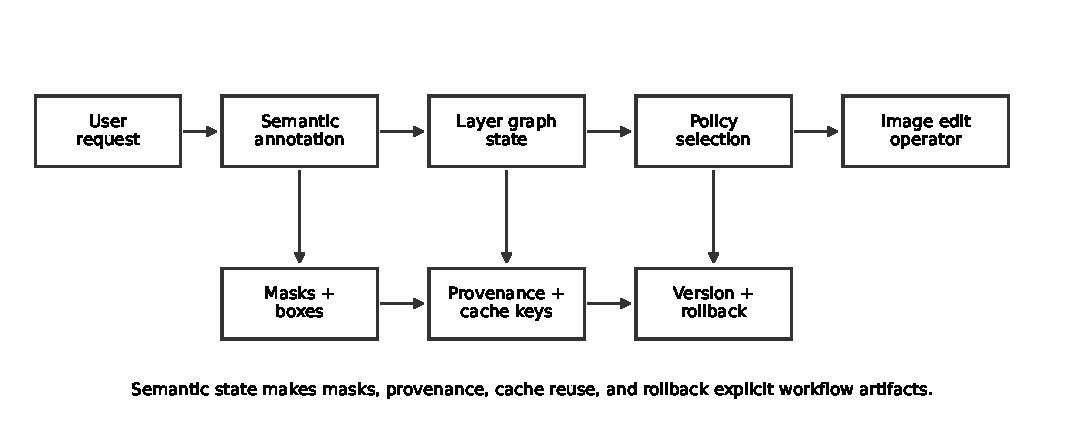
\includegraphics[width=0.95\textwidth]{figures/workflow_architecture.pdf}
    \caption{Semantic layer workflow architecture. The key difference from a monolithic diffusion call is that semantic annotation, layer graph state, cache keys, and version provenance are first-class workflow artifacts.}
    \label{fig:architecture}
\end{figure*}

\subsection{Semantic Image DOM}

The \imageDOM{} is the persistent state that makes repeated edits efficient. For each layer, it stores the mask, bounding box, label, detector backend, detector confidence where available, crop geometry, parent/child relations, and edit history. It also stores global provenance: model checkpoint name, scheduler, inference steps, seed, image size, guidance scale, and prompt. The representation is intentionally close to workflow provenance models: it records entities, activities, and derivations rather than only final pixels \citep{moreau2013prov}.

The current prototype uses file-system persistence for simplicity. Each sample output folder contains the base image, detector mask overlay, naive edit outputs, semantic local outputs, projection-only output, rollback output, sample grid, and a metrics record. This is sufficient for reproducible experiments. A production implementation would replace this with a content-addressed store or workflow database.

\subsection{Detector and mask stage}

The heavy benchmark uses GroundingDINO for open-vocabulary target localization and SAM2 for mask generation. The target labels are selected from the edit category: lips for face edits, shirt for body edits, mug for object edits, and sky for landscape edits. The detector stage returns a mask and bounding box. The local renderer expands the bounding box with padding and snaps to a crop size supported by the model backend.

Detector time is included as a separate metric because semantic annotation is expensive enough to change the conclusion. A one-off edit with no cached layer state may be slower than naive generation, while a repeated edit on the same layer avoids detection and becomes much faster.

\subsection{Execution policy}

The prototype policy is rule-based but grounded in the cost model above. Projection-only is selected for deterministic color changes when the target layer is already known. Semantic local diffusion is selected when the edit requires generative texture or lighting. Cached re-edit is selected when the layer mask and crop state already exist. Naive regeneration is used as the baseline and remains appropriate for global, structural, or highly entangled edits.

\begin{quote}
\small
\textbf{Algorithm 1: Rule-based semantic workflow policy.}

\begin{enumerate}[leftmargin=*]
    \item Input edit \(e=(q,a,s,\kappa)\), candidate layers \(V\), context \(C\), and version state.
    \item Resolve \(q\) to a target layer \(\ell_i\), or run detector inference if no matching layer exists.
    \item Construct feasible operators \(\mathcal{O}_{\mathrm{feasible}}\): rollback, projection, cached local edit, first local edit, and full regeneration.
    \item Remove operators that violate hard constraints, such as unavailable cache, privacy restrictions, unsupported model family, or missing mask.
    \item Estimate \(\widehat{T}_o\), \(\widehat{D}_o\), \(\widehat{Q}_o\), \(\widehat{U}_o\), and \(\widehat{R}_o\) from layer geometry, cache state, detector status, crop size, and benchmarked model family.
    \item Prefer rollback for undo, projection for simple deterministic color edits, cached local editing for repeated local variants, first local editing when preservation is required, and full regeneration for global or highly entangled edits.
    \item If more than one operator remains plausible, return the feasible operator with the lowest \(J(o \mid e,\ell_i,C)\).
\end{enumerate}
\end{quote}

Figure~\ref{fig:policy} gives a conceptual view of the operator space. The boundary between regions is not fixed; it depends on detector availability, cache state, latency budget, crop size, and quality requirements. This is why we report both generation-only and detector-inclusive speedups.

\begin{figure}[t]
    \centering
    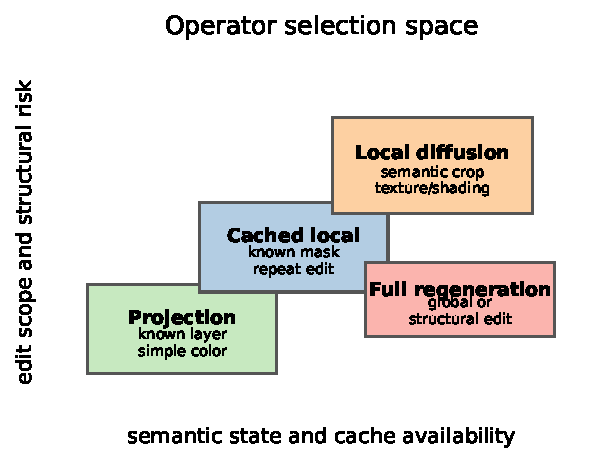
\includegraphics[width=0.98\columnwidth]{figures/policy_space.pdf}
    \caption{Conceptual operator selection space. Simple local edits favor deterministic projection or cached local rendering, while structurally broad edits may require full regeneration.}
    \label{fig:policy}
\end{figure}

\subsection{Implementation and artifact layout}

The prototype is implemented as Python scripts around local Hugging Face Diffusers pipelines and local model checkpoints \citep{huggingfaceDiffusers}. The heavy benchmark driver creates a resumable output directory and appends a JSON record after every completed sample. This design was important in practice because SDXL model transitions can fragment MPS memory; a resumed process can skip completed records and continue from the next missing model/case/sample tuple.

Each sample directory follows the same structure:
\begin{verbatim}
sample_XX/
  base.png
  mask_overlay.png
  naive_v1.png
  naive_v2.png
  semantic_raw_v1.png
  semantic_projected_v1.png
  semantic_cached_v2.png
  projection_only.png
  rollback.png
  sample_grid.png
  metrics.json
\end{verbatim}
The exact filenames vary slightly by operator, but the invariant is that every image artifact is paired with a metrics record. The aggregate directory contains a full JSON file, a Markdown report, a model-case CSV matrix, and representative sample grids. This layout is intentionally simple: it can be inspected without a database, archived with the paper, or converted into a formal workflow provenance store.

The policy engine is therefore a transparent heuristic scheduler rather than an optimized solver. This is a deliberate prototype choice: the experiment first tests whether the \imageDOM{} exposes useful scheduling features. The parameters \(\alpha,\beta,\gamma,\delta,\eta\) can later be fitted from user preferences, measured energy, or deployment constraints, but the current paper reports the rule-based policy and the cost-model simulations separately.

\subsection{Failure handling}

Long-running generative workflows benefit from partial-failure tolerance. The benchmark treats each sample tuple as an idempotent unit identified by model key, case key, and sample index. If execution stops after writing a record, the next run skips that tuple. This allowed the local benchmark to retain progress after memory-related restarts.

\section{Experimental Methodology}

\subsection{Research questions}

The evaluation is organized around eight questions:

\begin{description}[leftmargin=*]
    \item[RQ1] Does semantic workflow execution reduce non-target drift compared with naive full-image regeneration?
    \item[RQ2] When detector overhead is excluded, does local semantic rendering reduce generation time?
    \item[RQ3] What is the first-edit latency when semantic detection is included?
    \item[RQ4] How much speedup is obtained from cached semantic re-edits and versioning?
    \item[RQ5] How does performance vary by model family and edit category?
    \item[RQ6] What trade-offs appear between deterministic projection, local diffusion, and full regeneration?
    \item[RQ7] How sensitive are scheduling conclusions to heterogeneous resource assumptions?
    \item[RQ8] Do perceptual and dependency-risk audits support the pixel-level preservation results?
\end{description}

\subsection{Benchmark design}

We ran a paired benchmark over 10 compatible local diffusion checkpoints, four edit categories, and five seed variants per category, for 200 paired samples. Each sample executes the same workflow pattern:

\begin{enumerate}[leftmargin=*]
    \item Generate or load a base image at \(768 \times 768\).
    \item Execute a naive full-image first edit.
    \item Execute a second naive variant edit.
    \item Detect the target semantic layer using GroundingDINO and SAM2.
    \item Execute projection-only deterministic editing.
    \item Execute semantic local diffusion on the target crop and composite through the mask.
    \item Execute a cached semantic re-edit using the same layer state.
    \item Execute rollback to a prior version.
    \item Save images, masks, sample grids, and metrics.
\end{enumerate}

All runs use 20 denoising steps. The four cases are face/lips color editing, human body/shirt editing, object/mug editing, and landscape/sky editing. These categories were chosen because they cover small facial parts, medium human regions, discrete objects, and broader background regions. The local rendering crop is determined from the SAM2 mask and may be smaller than the full image, but it is padded and quantized for model compatibility.

The benchmark ran on the local workstation using the available Apple MPS backend. Some SDXL model transitions required process restart because of MPS memory fragmentation; the benchmark is resumable and persisted completed records were reused rather than recomputed. This is reported as part of the realistic local execution environment, not hidden as a failure. The final benchmark completed 200 samples with zero per-sample errors. Four incompatible local checkpoint files were excluded because they were inpainting-only, SD3, non-image-generation, or incomplete checkpoint entries.

To reduce the hardware-specificity threat, we also ran measured CUDA experiments on Google Cloud Platform. The main cloud run uses a \(g2\)-standard-8 VM with one NVIDIA L4 GPU and Juggernaut X RunDiffusion from the project model bucket, corresponding to the RunDiffusion Juggernaut X v10 model-card family \citep{hfJuggernautXV10}. It reruns the detector-inclusive workflow for 100 samples across the same four edit categories. A second L4 experiment sweeps denoising steps \(\{10,20,30\}\) and crop sizes \(\{256,384,512,640,768\}\), yielding 45 operator timing samples. A compact NVIDIA T4 tier repeats the 20-step operator measurement with CPU offload and VAE tiling. Finally, a long-session L4 benchmark runs repeated edit sessions across Juggernaut X, SDXL Base 1.0, DreamShaper XL, DreamShaper 8, and OpenJourney v4. Each session first annotates the target once and then runs enough full-image and semantic local variants to produce 5--10 minutes of naive generation work. These cloud experiments are still not a full multi-tier scheduler, but they provide measured accelerator evidence rather than relying only on scaled local timings.

\subsection{Models}

Table~\ref{tab:models} lists the 10 compatible checkpoints. The set intentionally includes both SD1.5-family and SDXL-family models because throughput and img2img cost differ substantially across families. The table reports the benchmark names used in the local output records; the corresponding public Hugging Face model-card identifiers are cited below the table where available.

\begin{table*}[t]
\centering
\small
\setlength{\tabcolsep}{5pt}
\caption{Evaluated diffusion checkpoints. Each model is evaluated on four edit categories with five seed variants per category.}
\label{tab:models}
\begin{tabular}{llrrrr}
\toprule
Model & Family & Samples & Naive (s) & Semantic local (s) & Detector (s) \\
\midrule
Deliberate v6 & SD1.5 & 20 & 12.213 & 8.180 & 12.954 \\
DreamShaper 8 & SD1.5 & 20 & 31.388 & 8.298 & 13.292 \\
DreamShaper XL 1.0 & SDXL & 20 & 39.873 & 55.469 & 14.677 \\
Juggernaut Reborn & SD1.5 & 20 & 11.390 & 4.973 & 12.778 \\
Juggernaut XL v2 & SDXL & 20 & 118.220 & 75.622 & 15.298 \\
OpenJourney v4 & SD1.5 & 20 & 23.941 & 7.496 & 12.384 \\
RealVisXL V4.0 & SDXL & 20 & 53.656 & 62.119 & 14.488 \\
Realistic Vision V6.0 B1 & SD1.5 & 20 & 10.540 & 9.139 & 12.194 \\
SDXL Base 1.0 & SDXL & 20 & 43.568 & 60.456 & 14.151 \\
Stable Diffusion 1.5 Base & SD1.5 & 20 & 10.675 & 9.567 & 13.220 \\
\bottomrule
\end{tabular}
\end{table*}

The baseline Stable Diffusion checkpoints correspond to the Stable Diffusion v1.5 and SDXL Base 1.0 model cards \citep{hfStableDiffusionV15,hfStableDiffusionXLBase}. The remaining rows cite the public model-card families used for provenance: DreamShaper \citep{hfDreamShaper8,hfDreamShaperXL}, OpenJourney v4 \citep{hfOpenJourneyV4}, Realistic Vision and RealVisXL \citep{hfRealisticVisionV6,hfRealVisXLV4}, Deliberate \citep{hfDeliberate}, Juggernaut Reborn \citep{hfJuggernautReborn}, and RunDiffusion Juggernaut XL \citep{hfJuggernautXLV2}. Since third-party model cards and licenses can change, the artifact records local checkpoint filenames and output metrics but does not redistribute weights.

\subsection{Metrics}

The benchmark records four groups of metrics.

\textbf{Latency metrics} include naive first-edit time, naive second-edit time, detector time, semantic local render time, cached semantic re-edit time, projection-only time, and rollback time. We report three speedup variants:
\begin{align}
    S_{\mathrm{gen}} &= T_{\mathrm{naive}} / T_{\mathrm{semantic}}, \\
    S_{\mathrm{incl}} &= T_{\mathrm{naive}} / (T_{\mathrm{det}} + T_{\mathrm{semantic}}), \\
    S_{\mathrm{cached}} &= T_{\mathrm{naive2}} / T_{\mathrm{cached}}.
\end{align}
\(S_{\mathrm{gen}}\) asks whether local rendering is faster than full rendering once a layer is known. \(S_{\mathrm{incl}}\) asks whether the first semantic edit is faster for a user with no cache. \(S_{\mathrm{cached}}\) asks whether repeated edits benefit from the persisted \imageDOM{}.

\textbf{Locality metrics} measure outside-target changed pixels, inside-target mean absolute difference, and boundary-band changed pixels. These quantify preservation and seam risk. The outside-target metric is especially important because full-image regeneration can be visually plausible while still destroying identity or layout.

\textbf{Layer geometry metrics} include mask area percentage, bounding-box area percentage, crop size, and crop-pixel percentage. These help explain why some local edits are faster than others.

\textbf{Perceptual metrics} include LPIPS full-image, outside-mask, and target-crop distances computed between the base image and each output variant. LPIPS is not a semantic-intent metric, but it tests whether the low-level preservation results also hold under a learned perceptual distance.

\textbf{Dependency-contact metrics} approximate layer dependency risk with a ring immediately outside the target mask. The metric measures how much the area most likely to contain neighboring structures changes after semantic compositing. It is a geometry-only proxy, not a replacement for attention-map or depth-based dependency edges.

\textbf{Versioning metrics} include cached re-edit time and rollback time. These directly test whether semantic state makes repeated edits and undo operations cheap.

\textbf{Resource proxy metrics} include crop-pixel percentage and detector invocation. These are not watt-level energy measurements. They instantiate the resource term \(\widehat{R}_o\) as relative diffusion area and detector work so that the scheduler can compare full rendering, local rendering, projection, and rollback on a common scale.

\subsection{Reproducibility artifacts}

The benchmark stores machine-readable results in JSON and CSV. The JSON contains all per-sample records and aggregate summaries. The CSV contains the model-by-case matrix used for compact comparison. Figures in this manuscript are generated from those files rather than manually transcribed. The manuscript directory also includes copied sample grids for the appendix. The most important reproducibility fields are model key, model family, case key, sample index, seed, image width/height, steps, mask area, bounding-box area, crop size, detector time, render times, speedups, drift metrics, and artifact directory.

The public artifact does not include model checkpoints or detector weights because those files are large and governed by separate licenses. It includes the scripts, reports, aggregate metrics, model-case matrix, manuscript source, and representative image artifacts needed to inspect the reported results.

\section{Results}

\subsection{Overall performance}

Table~\ref{tab:overall} summarizes the full 200-sample benchmark. Semantic local rendering excluding detector cost is faster than naive full-image generation on average. However, detector-inclusive first edits are slower on average. Cached re-edits are the strongest performance result, with a 7.041x average speedup. Projection-only edits are effectively instantaneous for simple color changes, and rollback is near-interactive.

\begin{table}[t]
\centering
\caption{Overall benchmark results across 200 paired executions.}
\label{tab:overall}
\begin{tabular}{lr}
\toprule
Metric & Mean \\
\midrule
Naive full edit time & 35.546 s \\
Semantic local edit time, detector excluded & 30.132 s \\
Detector time & 13.543 s \\
Projection-only edit time & 0.031 s \\
Generation-only semantic speedup & 1.788x \\
One-off detector-inclusive speedup & 0.809x \\
Cached version re-edit speedup & 7.041x \\
Projection-only speedup & 1227.276x \\
Rollback time & 0.188 s \\
Naive outside-target changed pixels & 93.954\% \\
Semantic outside-target changed pixels & 0.000\% \\
Semantic boundary-band changed pixels & 42.301\% \\
Mean crop-pixel work proxy & 42.145\% \\
Mean mask area & 6.032\% \\
\bottomrule
\end{tabular}
\end{table}

The detector-inclusive number is the first-edit result. When a user edits a region for the first time and the system has no cached semantic layer, GroundingDINO+SAM2 adds substantial overhead. This overhead can be justified when preservation matters, but it does not guarantee lower latency. Once the semantic layer exists, repeated variants avoid detection and reuse the layer state.

\subsection{Baseline decomposition}

Table~\ref{tab:baseline-decomp} separates the benchmark into operator-level baselines. This comparison is important because the workflow is not only evaluated against full-image regeneration. The detector-inclusive local edit represents an ordinary first local edit with semantic detection but no reuse. Known-mask local rendering removes detector cost. Cached re-editing then measures the additional value of persisted workflow state.

\begin{table}[t]
\centering
\scriptsize
\caption{Operator-level baseline decomposition across 200 samples.}
\label{tab:baseline-decomp}
\begin{tabular}{lr}
\toprule
Operator & Mean time \\
\midrule
Naive full regeneration & 35.546 s \\
Detector + local semantic edit & 43.675 s \\
Known-mask local rendering & 30.132 s \\
Cached semantic re-edit & 8.115 s \\
Deterministic projection & 0.031 s \\
Rollback & 0.188 s \\
\bottomrule
\end{tabular}
\end{table}

The decomposition shows why caching is central to the contribution. The first detector-inclusive local edit is slower than full regeneration on average, but known-mask local rendering is faster, and cached semantic re-editing is 5.382x faster than the detector-inclusive local baseline. The workflow gain therefore comes from making semantic state persistent and reusable, not from assuming that every local edit is automatically faster than a full-image edit.

\subsection{Edit category effects}

Table~\ref{tab:cases} and Figure~\ref{fig:case-speedups} show results by edit category. Face/lips edits have the highest cached speedup at 11.055x because the editable region is small and repeated color changes are cheap. Human body/shirt and object/mug edits show similar cached speedups near 6x. Landscape/sky edits are less favorable because the semantic region and crop are often larger, but cached re-editing still averages 4.966x.

\begin{table*}[t]
\centering
\scriptsize
\setlength{\tabcolsep}{3.5pt}
\caption{Results by edit category. Each category contains 50 paired samples.}
\label{tab:cases}
\begin{tabular}{lrrrrrrrr}
\toprule
Case & Naive & Local & Det. & Gen. & Incl. & Cached & Naive drift & Sem. drift \\
\midrule
Face lips & 35.796 & 28.063 & 13.871 & 2.313x & 0.877x & 11.055x & 90.355\% & 0.000\% \\
Human body shirt & 38.372 & 30.619 & 13.517 & 1.958x & 0.886x & 6.085x & 91.908\% & 0.000\% \\
Landscape sky & 31.858 & 31.358 & 13.636 & 1.211x & 0.634x & 4.966x & 98.745\% & 0.000\% \\
Object mug & 36.160 & 30.488 & 13.151 & 1.669x & 0.838x & 6.058x & 94.809\% & 0.000\% \\
\bottomrule
\end{tabular}
\end{table*}

\begin{figure}[t]
    \centering
    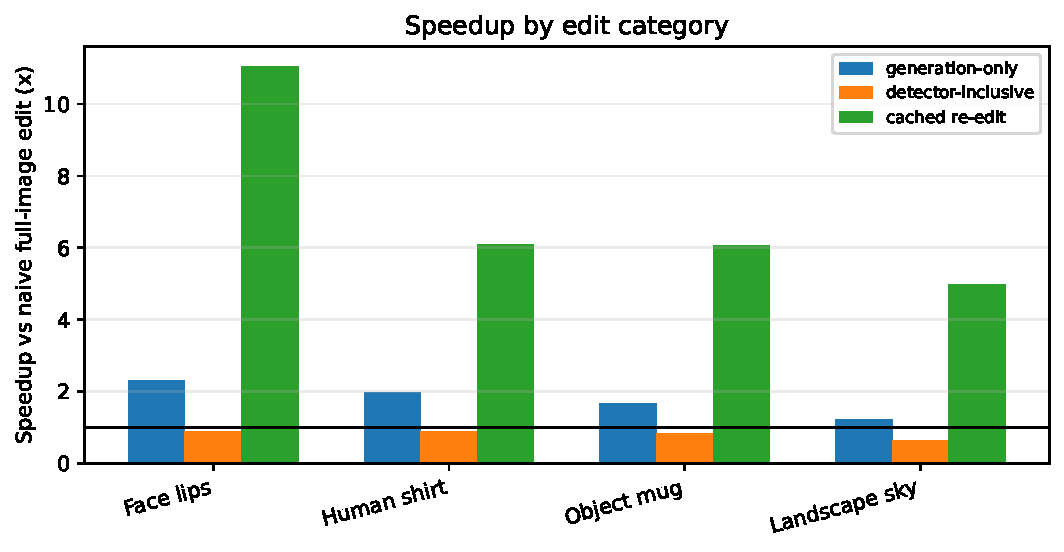
\includegraphics[width=0.98\columnwidth]{figures/speedups_by_case.pdf}
    \caption{Speedup by edit category. Cached semantic re-edit is positive for all categories, while detector-inclusive first-edit speedup is below 1x on average.}
    \label{fig:case-speedups}
\end{figure}

These results support a policy-based interpretation. If the target is small and the edit is simple, projection-only or cached local editing is attractive. If the target is broad, first-edit performance may not improve, but preservation can still justify semantic execution. Layer geometry and cache state are therefore useful scheduling features.

\subsection{Model effects}

Figure~\ref{fig:model-speedups} shows strong model dependence. DreamShaper 8, OpenJourney v4, and Juggernaut XL v2 achieve detector-inclusive first-edit speedups above 1x. Other models, especially several SDXL checkpoints, are slower in the semantic first-edit path. This occurs because local img2img throughput and full-generation throughput differ by checkpoint and pipeline implementation. It would be misleading to claim that local semantic rendering is always faster. To make the non-SDXL evidence explicit, Table~\ref{tab:top5-models} reports the five strongest models ranked by cached semantic re-edit speedup from the completed 200-sample benchmark. Four of these five are SD1.5-family checkpoints.

\begin{figure*}[t]
    \centering
    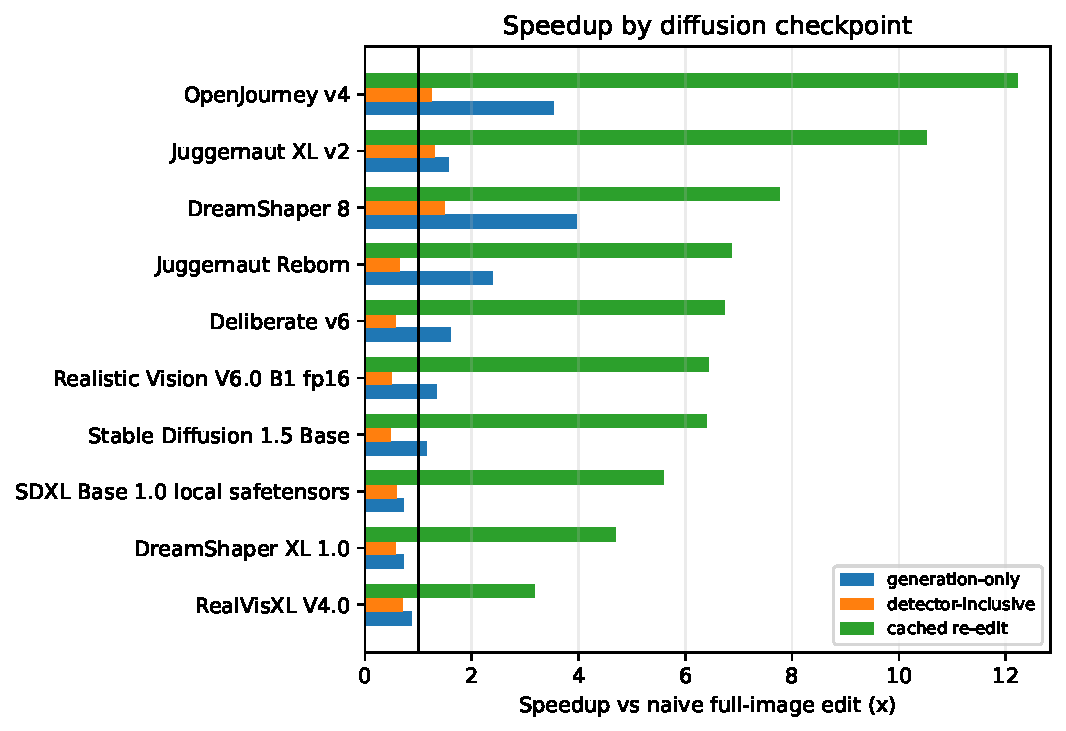
\includegraphics[width=0.95\textwidth]{figures/speedups_by_model.pdf}
    \caption{Speedup by model. The generation-only metric isolates local rendering cost; the detector-inclusive metric represents first-edit user latency; cached re-edit represents repeated semantic layer editing.}
    \label{fig:model-speedups}
\end{figure*}

\begin{table*}[t]
\centering
\scriptsize
\caption{Top-five cross-model results from the 200-sample local heavy benchmark, ranked by cached semantic re-edit speedup. Each row aggregates 20 paired executions: four edit categories with five seeds each.}
\label{tab:top5-models}
\begin{tabular}{llrrrrrrr}
\toprule
Rank & Model & Family & Naive & Local & Detector & Cached & Gen. & Incl. / cached \\
\midrule
1 & OpenJourney v4 & SD1.5 & 23.941 & 7.496 & 12.384 & 3.618 & 3.537x & 1.246x / 12.229x \\
2 & Juggernaut XL v2 & SDXL & 118.220 & 75.622 & 15.298 & 26.529 & 1.567x & 1.303x / 10.514x \\
3 & DreamShaper 8 & SD1.5 & 31.388 & 8.298 & 13.292 & 4.883 & 3.970x & 1.483x / 7.762x \\
4 & Juggernaut Reborn & SD1.5 & 11.390 & 4.973 & 12.778 & 2.109 & 2.392x & 0.643x / 6.872x \\
5 & Deliberate v6 & SD1.5 & 12.213 & 8.180 & 12.954 & 2.610 & 1.601x & 0.579x / 6.744x \\
\bottomrule
\end{tabular}
\end{table*}

The workflow conclusion remains stable across models: cached re-editing is positive for every checkpoint. The weakest cached result is RealVisXL V4.0 at 3.172x, while the strongest is OpenJourney v4 at 12.229x. The top-five table also shows why the policy cannot use model family alone: DreamShaper 8 and OpenJourney v4 are strong detector-inclusive first-edit cases, while Juggernaut Reborn and Deliberate v6 are faster mainly when detector state is reused. This suggests that semantic caching is a robust systems mechanism even when first-edit acceleration is model-dependent.

\subsection{Locality and drift}

Naive full-image regeneration changes an average of 93.954\% of outside-target pixels. Semantic compositing changes 0.000\% outside-target pixels under the exact pixel-change metric because the edited crop is composited through the semantic mask and the unmasked base image is preserved.

This metric is intentionally strict. It does not claim that semantic edits are always perceptually superior; it shows that the workflow preserves non-target pixels by construction. This is useful when identity, layout, text, object positions, or scientific visual state must remain stable. The boundary-band change average of 42.301\% indicates that changes occur near seams, so visual seam quality still requires inspection and better blending methods.

\subsection{Trade-offs}

The main trade-off is between first-edit latency and state reuse. Semantic editing pays an annotation cost before it can exploit locality. In the benchmark, this cost is large enough that the first detector-inclusive edit is slower than naive regeneration on average. This is acceptable when the user expects to make several changes to the same region, compare variants, or preserve the surrounding image exactly. It is less attractive for a single low-stakes edit where global regeneration is visually acceptable and latency is the only concern.

The second trade-off is between preservation and visual integration. Mask compositing keeps non-target pixels fixed, which is useful for identity, layout, text, product images, or scientific visual state. The same constraint can make boundaries more visible if the local edit changes lighting, texture, or geometry near the mask edge. In those cases, semantic execution is still useful as a controlled editing mode, but it should be paired with better blending, boundary-aware scoring, or a policy that expands the crop when the edit is structurally coupled to nearby regions.

A third trade-off is implementation complexity. Maintaining masks, cache keys, provenance, and version state is more work than calling a diffusion pipeline once. The benefit appears when edits are iterative, audited, or reused: cached re-edits become faster, rollback is cheap, and the system can explain which model, mask, crop, and parameters produced each result. For casual one-shot generation this overhead may not be justified; for repeated editing workflows it becomes the mechanism that makes locality and reproducibility practical.

\subsection{Versioning and rollback}

Rollback averages 0.188 s. This supports the versioning model: undoing a semantic edit restores cached state rather than invoking diffusion. In interactive workflows, rollback changes the editing process from destructive regeneration to a versioned exploration tree. Users can compare variants of the same object while preserving the rest of the image and retaining intermediate states.

The cached re-edit result is similarly important. A first semantic edit may be slower because of detector overhead, but subsequent edits amortize semantic annotation. This is analogous to scientific workflows where expensive preprocessing or indexing steps become worthwhile when reused across many downstream tasks.

\subsection{Scheduling-policy simulation}

Table~\ref{tab:policy-sim} applies a simple scheduling simulation to the 200 measured records. For a session with \(k\) edits on the same layer, the naive policy uses full regeneration for every variant, the semantic policy pays detector cost once and then uses cached re-edits, and the oracle latency policy chooses the faster of the two measured paths per sample. This is not a new deployment experiment, but it evaluates the scheduling decision that the workflow representation exposes.

\begin{table}[t]
\centering
\scriptsize
\caption{Measured scheduling-policy simulation. \(k\) is the number of edits on the same semantic layer. Times are mean seconds across 200 samples.}
\label{tab:policy-sim}
\begin{tabular}{rrrrr}
\toprule
\(k\) & Naive & Semantic & Oracle & Sem. wins \\
\midrule
1 & 35.546 & 43.675 & 30.780 & 25.5\% \\
2 & 71.287 & 51.791 & 49.543 & 60.0\% \\
3 & 107.027 & 59.906 & 59.839 & 98.0\% \\
5 & 178.509 & 76.137 & 75.967 & 99.5\% \\
\bottomrule
\end{tabular}
\end{table}

The policy result is stronger than the mean break-even calculation because it shows how often each decision is preferred across heterogeneous models and edit categories. For \(k=1\), semantic editing is not a latency default. For \(k=2\), reuse already changes the decision for most samples. For \(k=5\), semantic execution is faster almost everywhere. This supports the systems claim that session context, cache state, and preservation constraints should be explicit scheduler inputs rather than hidden inside a single image-generation call.

Table~\ref{tab:policy-ablation} further separates latency-only scheduling from preservation-aware scheduling. The latency-only policy selects semantic execution only when it is faster for the current sample and session length. The preservation-first policy always selects semantic execution when a target mask exists, because outside-target stability is treated as a hard requirement. The balanced policy uses latency when \(k=1\), but selects semantic execution for repeated edits because cache reuse and outside preservation dominate after the first edit. The oracle column is the measured faster path and is included only as a latency reference.

\begin{table*}[t]
\centering
\scriptsize
\caption{Policy ablation over the 200 measured records. Latency is mean seconds for the \(k\)-edit session; drift is mean outside-target drift.}
\label{tab:policy-ablation}
\begin{tabular}{llrrr}
\toprule
\(k\) & Policy & Semantic selected & Latency & Outside drift \\
\midrule
1 & Latency-only / oracle & 25.5\% & 30.780 & 69.973\% \\
1 & Preservation-first & 100.0\% & 43.675 & 0.000\% \\
1 & Balanced & 25.5\% & 30.780 & 69.973\% \\
2 & Latency-only / oracle & 60.0\% & 49.543 & 38.102\% \\
2 & Preservation-first & 100.0\% & 51.791 & 0.000\% \\
2 & Balanced & 100.0\% & 51.791 & 0.000\% \\
3 & Latency-only / oracle & 98.0\% & 59.839 & 1.773\% \\
3 & Preservation-first & 100.0\% & 59.906 & 0.000\% \\
3 & Balanced & 100.0\% & 59.906 & 0.000\% \\
5 & Latency-only / oracle & 99.5\% & 75.967 & 0.455\% \\
5 & Preservation-first & 100.0\% & 76.137 & 0.000\% \\
5 & Balanced & 100.0\% & 76.137 & 0.000\% \\
\bottomrule
\end{tabular}
\end{table*}

The ablation exposes the role of the objective weights without claiming that the prototype learns them. If latency is the only objective, semantic execution is not a universal first-edit choice. If preservation is a hard constraint, the semantic path is chosen even when it is slower. If the session contains repeated edits, the balanced rule converges to semantic execution because the detector cost is amortized and the non-target preservation gain is large. This bridges the cost model and the implemented rule engine: the current system evaluates a transparent finite set of policies rather than solving a learned optimization problem.

\subsection{Heterogeneous resource sensitivity}

The measured benchmark uses Apple MPS, so the absolute detector and diffusion times should not be treated as universal. To test whether the scheduling conclusion depends only on this desktop configuration, Table~\ref{tab:hetero-sim} applies a sensitivity model to the 200 measured records. The model scales detector time and diffusion time separately:
\begin{align}
    T^{r}_{\mathrm{naive}} &= s^r_{\mathrm{diff}} T_{\mathrm{naive}} + L^r, \\
    T^{r}_{\mathrm{sem}} &= s^r_{\mathrm{det}}T_{\mathrm{det}} + s^r_{\mathrm{diff}}T_{\mathrm{local}} + L^r, \\
    T^{r}_{\mathrm{cached}} &= s^r_{\mathrm{diff}}T_{\mathrm{cached}} + L^r,
\end{align}
where \(s^r_{\mathrm{det}}\) and \(s^r_{\mathrm{diff}}\) are resource-tier scaling factors and \(L^r\) is a transfer or orchestration penalty. The factors are not presented as measurements of named commercial hardware; they are stress-test scenarios that represent slower edge execution, the measured local run, faster CUDA-class execution, and a cloud accelerator with transfer overhead.

\begin{table*}[t]
\centering
\small
\caption{Heterogeneous resource sensitivity projection using the 200 measured records. Times are projected mean seconds. \(k=3\) denotes three edits on the same semantic layer.}
\label{tab:hetero-sim}
\begin{tabular}{lrrrrrr}
\toprule
Scenario & \(s_{\mathrm{det}}\) & \(s_{\mathrm{diff}}\) & Naive \(k=1\) & Semantic \(k=1\) & Semantic speed & \(k=3\) speed \\
\midrule
Edge-constrained & 1.80 & 1.50 & 53.320 & 69.576 & 0.766x & 1.709x \\
Measured Apple MPS & 1.00 & 1.00 & 35.546 & 43.675 & 0.814x & 1.787x \\
CUDA workstation & 0.35 & 0.45 & 15.996 & 18.300 & 0.874x & 1.881x \\
Cloud accelerator, \(L=1.5\) s & 0.15 & 0.20 & 8.609 & 9.558 & 0.901x & 1.639x \\
\bottomrule
\end{tabular}
\end{table*}

The projection preserves the main conclusion but changes its magnitude. Faster accelerators reduce both full-generation and local-diffusion latency, while faster detectors narrow the first-edit penalty. In all four scenarios, the one-off semantic path remains slower on average, but the three-edit session is faster because detection is amortized and cached re-edits are cheap. This is the compute-continuum claim supported by the present evidence: the exact break-even point is resource dependent, but the \imageDOM{} exposes the variables a placement scheduler needs to recompute the decision.

Table~\ref{tab:l4-detector-bench} reports the measured detector-inclusive CUDA tier. Unlike the earlier operator-only run, this experiment executes GroundingDINO+SAM2 on the L4 for every sample. The detector is loaded once, and warm per-sample detector inference averages 0.235 s. Full-image naive editing averages 4.882 s, local semantic diffusion averages 0.939 s, and the detector-inclusive semantic path averages 1.174 s. The resulting detector-inclusive speedup is 4.28x, while cached re-edits average 5.52x. This directly changes the interpretation of the local Apple MPS result: the first-edit penalty is not inherent to the workflow model, but depends on the relative speed of detector inference and diffusion on the chosen resource tier.

\begin{table}[t]
\centering
\scriptsize
\caption{Measured detector-inclusive SDXL workflow benchmark on GCP NVIDIA L4. The run uses 100 samples across four edit categories at 20 denoising steps.}
\label{tab:l4-detector-bench}
\begin{tabular}{lr}
\toprule
Metric & Value \\
\midrule
Samples completed & 100 \\
Naive full-image edit & 4.882 s \\
Detector inference & 0.235 s \\
Semantic local diffusion & 0.939 s \\
Detector-inclusive semantic edit & 1.174 s \\
Cached local re-edit & 0.931 s \\
Generation-only speedup & 5.45x \\
Detector-inclusive speedup & 4.28x \\
Cached speedup & 5.52x \\
Naive outside-mask drift & 85.009\% \\
Semantic outside-mask drift & 0.000\% \\
\bottomrule
\end{tabular}
\end{table}

Table~\ref{tab:l4-sweep} reports the larger L4 operator sweep. It shows the expected dependency between crop area and speedup: small and medium crops benefit most, while a \(768 \times 768\) img2img pass is still faster than full txt2img in this configuration but no longer represents a locality win. Across 45 timing samples, mean operator speedup is 4.42x and median speedup is 5.08x. At the paper's 20-step setting, \(384 \times 384\) and \(512 \times 512\) crops achieve 6.18x and 5.17x speedup, respectively.

\begin{table}[t]
\centering
\scriptsize
\caption{GCP NVIDIA L4 crop/step operator sweep. Each condition has three repeats. Area is relative to a \(768 \times 768\) full image.}
\label{tab:l4-sweep}
\begin{tabular}{rrrrr}
\toprule
Steps & Crop & Area & Full & Local / speedup \\
\midrule
10 & 256 & 11.1\% & 2.662 & 0.461 / 5.82x \\
10 & 384 & 25.0\% & 2.662 & 0.535 / 4.99x \\
10 & 512 & 44.4\% & 2.662 & 0.681 / 3.91x \\
20 & 256 & 11.1\% & 4.988 & 0.722 / 6.91x \\
20 & 384 & 25.0\% & 4.988 & 0.807 / 6.18x \\
20 & 512 & 44.4\% & 4.988 & 0.965 / 5.17x \\
20 & 640 & 69.4\% & 4.988 & 1.539 / 3.24x \\
30 & 384 & 25.0\% & 7.074 & 1.183 / 5.98x \\
30 & 512 & 44.4\% & 7.074 & 1.360 / 5.20x \\
\bottomrule
\end{tabular}
\end{table}

Table~\ref{tab:t4-tier} adds a compact T4 tier. The T4 required CPU offload and VAE tiling to avoid out-of-memory failures with both SDXL pipelines. Under that constrained execution mode, the 20-step full-image edit averages 16.658 s and local crops average 7.882 s, giving 2.21x mean speedup. This is slower than the L4 tier, but it is still useful: it shows that memory capacity and pipeline residency are scheduling variables, not incidental implementation details.

\begin{table}[t]
\centering
\scriptsize
\caption{Compact GCP NVIDIA T4 operator tier with CPU offload and VAE tiling. Each condition has two repeats at 20 denoising steps.}
\label{tab:t4-tier}
\begin{tabular}{rrrrr}
\toprule
Crop & Area & Full & Local & Speedup \\
\midrule
384 & 25.0\% & 16.658 & 7.929 & 2.26x \\
512 & 44.4\% & 16.658 & 6.526 & 2.55x \\
768 & 100.0\% & 16.658 & 9.192 & 1.81x \\
\midrule
All samples & -- & 16.658 & 7.882 & 2.21x \\
\bottomrule
\end{tabular}
\end{table}

Table~\ref{tab:heavy-session} reports the long-session L4 benchmark. Unlike the short per-image timing runs, this experiment measures repeated user-like edit sessions: one target annotation followed by many variant edits on the same semantic layer. The benchmark covers five model families and two target types. It executes 303 requested variants, totaling 2786.7 s of naive full-image regeneration and 528.9 s of detector-inclusive semantic execution. Mean detector-inclusive session speedup is 5.37x, with a range from 4.87x to 6.03x. The result strengthens the amortization claim: when the editing task is an exploratory session rather than a single isolated call, semantic state converts detector and mask cost into a small fixed overhead.

\begin{table}[t]
\centering
\scriptsize
\caption{Long GCP NVIDIA L4 edit-session benchmark. Each row runs one target annotation followed by repeated variants until the naive full-image session lasts about 5--10 minutes.}
\label{tab:heavy-session}
\begin{tabular}{llrrrr}
\toprule
Model & Case & Variants & Naive & Semantic & Speedup \\
\midrule
Juggernaut X & Mug & 45 & 641.4 & 131.0 & 4.90x \\
Juggernaut X & Shirt & 44 & 628.9 & 120.4 & 5.22x \\
SDXL Base 1.0 & Mug & 21 & 300.2 & 61.7 & 4.87x \\
DreamShaper XL & Mug & 21 & 300.5 & 54.1 & 5.55x \\
DreamShaper 8 & Mug & 58 & 305.6 & 54.4 & 5.62x \\
DreamShaper 8 & Shirt & 58 & 305.8 & 50.7 & 6.03x \\
OpenJourney v4 & Mug & 56 & 304.3 & 56.5 & 5.38x \\
\midrule
All sessions & -- & 303 & 2786.7 & 528.9 & 5.37x \\
\bottomrule
\end{tabular}
\end{table}

The project bucket also contains Flux, Wan, Qwen, Z-image, GGUF, and ComfyUI-specific weights. A runtime audit found 189 model objects: one directly measured SDXL checkpoint in the paper runtime, 52 objects requiring a separate runtime family, five GGUF objects that are not comparable under the SDXL Diffusers path, and 131 non-checkpoint or manually triaged objects. For this reason, the paper reports the bucket audit as a reproducibility and scope result rather than claiming a direct multi-model parity benchmark across incompatible runtimes.

Table~\ref{tab:stress-sim} adds a break-even stress test. Under the measured Apple MPS profile, the median break-even session length is \(k=1.79\), and 98.0\% of samples prefer semantic execution by \(k=3\). The result remains strong for CUDA-class and cloud-accelerator scenarios. In the adverse slow-detector/fast-diffusion case, median break-even increases to \(k=5.55\), and only 24.0\% of three-edit sessions prefer semantic execution. This defines where the policy should avoid local semantic execution unless preservation, provenance, or privacy dominates latency.

\begin{table}[t]
\centering
\scriptsize
\caption{Break-even stress test across resource assumptions. \(k=n\) columns report the percentage of samples where semantic execution is faster by session length \(n\).}
\label{tab:stress-sim}
\begin{tabular}{lrrrr}
\toprule
Scenario & Median \(k^*\) & \(k=1\) & \(k=3\) & \(k=5\) \\
\midrule
Edge-constrained & 2.02 & 24.0\% & 92.5\% & 99.5\% \\
Measured Apple MPS & 1.79 & 25.5\% & 98.0\% & 99.5\% \\
CUDA-class & 1.61 & 26.5\% & 99.5\% & 99.5\% \\
Cloud accelerator & 1.58 & 26.5\% & 99.5\% & 99.5\% \\
Fast detector, slow diffusion & 0.89 & 54.0\% & 100.0\% & 99.5\% \\
Slow detector, fast diffusion & 5.55 & 0.0\% & 24.0\% & 46.0\% \\
\bottomrule
\end{tabular}
\end{table}

\subsection{Interpreting boundary-band change}

The average semantic boundary-band change is 42.301\%. This is not a failure rate: the band lies near the mask edge, where color, lighting, and antialiasing changes are expected after compositing. The benchmark treats boundary change as a seam-risk proxy for comparison and triage, not as a perceptual quality score.

\subsection{Automatic quality-risk audit}

Table~\ref{tab:quality-audit} adds an automatic quality-risk audit over the 200 samples. It does not replace human evaluation; it checks target confidence, edit activity, and seam risk using detector score, inside-target change, and boundary-band change.

\begin{table}[t]
\centering
\scriptsize
\caption{Automatic quality-risk audit across 200 samples. Thresholds are used only as triage flags.}
\label{tab:quality-audit}
\begin{tabular}{lrrr}
\toprule
Metric & Mean & Median & Flagged \\
\midrule
Detector selection score & 0.456 & 0.473 & 10.5\% below 0.25 \\
Inside-target change & 34.435 & 34.459 & 3.5\% below 20 \\
Boundary-band change & 42.301 & 42.825 & 3.0\% above 50 \\
\bottomrule
\end{tabular}
\end{table}

Most runs produced measurable target-region changes; a smaller subset should be inspected for weak detection or seam risk. Detector confidence and pixel-change metrics cannot prove user-intent satisfaction, but they provide reproducible triage for human or model-assisted perceptual scoring.

\subsection{Perceptual validation layer}

Pixel metrics are insufficient for final quality assessment. The evaluation therefore separates systems metrics from perceptual validation. As an immediate check, we compute full-image, outside-mask, and target-crop LPIPS between the base image and all 800 output variants. Table~\ref{tab:lpips-results} reports the aggregate result.

\begin{table}[t]
\centering
\scriptsize
\caption{LPIPS perceptual-distance audit over 800 output images. Lower outside-mask LPIPS indicates better perceptual preservation outside the target mask.}
\label{tab:lpips-results}
\begin{tabular}{lrrr}
\toprule
Variant & Full image & Outside mask & Target crop \\
\midrule
Naive regeneration & 0.5848 & 0.5614 & 0.7062 \\
Semantic local & 0.0364 & 0.0005 & 0.2847 \\
Cached semantic & 0.0283 & 0.0005 & 0.2244 \\
Projection-only & 0.0339 & 0.0004 & 0.2403 \\
\bottomrule
\end{tabular}
\end{table}

The cloud detector-inclusive run was also scored with LPIPS (Table~\ref{tab:cloud-lpips-results}). Because all cloud samples use the same SDXL checkpoint and compositing path, the locality pattern is stronger: naive regeneration has outside-mask LPIPS 0.4801, while semantic and cached outputs remain near zero at 0.00019. Target-crop scores remain non-zero, as expected for local edits.

\begin{table}[t]
\centering
\scriptsize
\caption{Cloud LPIPS audit over the 100-sample GCP L4 detector-inclusive run. The table reports 300 variant comparisons: naive, semantic, and cached outputs for each sample.}
\label{tab:cloud-lpips-results}
\begin{tabular}{lrrr}
\toprule
Variant & Full image & Outside mask & Target crop \\
\midrule
Naive regeneration & 0.5266 & 0.4801 & 0.6714 \\
Semantic local & 0.0085 & 0.0002 & 0.0895 \\
Cached semantic & 0.0071 & 0.0002 & 0.0802 \\
\bottomrule
\end{tabular}
\end{table}

Together, the LPIPS audits support the locality result with a learned perceptual metric. Naive regeneration has high full-image and outside-mask distance because the whole image is resampled; semantic, cached, and projection outputs keep outside-mask LPIPS near zero through compositing. LPIPS does not prove semantic success, but shows that preservation is not an artifact of a single pixel threshold.

Table~\ref{tab:perceptual-layer} defines the remaining validation layer for a production scheduler or follow-up benchmark; CLIP/BLIP alignment and human ratings are future semantic-quality checks.

\begin{table}[t]
\centering
\scriptsize
\caption{Perceptual validation layer for semantic editing quality.}
\label{tab:perceptual-layer}
\begin{tabular}{@{}p{0.27\columnwidth}p{0.27\columnwidth}p{0.30\columnwidth}@{}}
\toprule
Metric & Tests & Policy use \\
\midrule
CLIP/BLIP alignment & prompt/edit intent & semantic success risk \\
LPIPS target distance & perceptual change & over/under-edit risk \\
LPIPS outside mask & perceptual preservation & identity/layout risk \\
Human seam rating & boundary artifacts & expand crop/blend \\
Human task rating & edit satisfaction & policy training label \\
\bottomrule
\end{tabular}
\end{table}

These metrics would change \(\widehat{Q}_o\): low outside drift with poor CLIP alignment should not be considered successful, and visible seams should trigger a larger crop, blending, or full regeneration. The pixel audit is a cheap screen; semantic alignment and realism require model-assisted scoring or human labels.

\subsection{Dependency-risk audit}

The dependency formulation is broader than the implementation: a complete layer graph should use mask overlap, attention overlap, depth ordering, and contact evidence. Because the prototype cannot reconstruct DAAM maps after generation, we add a geometry-only audit. For each sample, a contact ring outside the target mask approximates where neighboring structures would reveal an over-tight crop or poor dependency expansion.

\begin{table}[t]
\centering
\scriptsize
\caption{Geometry-only dependency-risk audit over 200 samples. Contact change is measured in the ring just outside the semantic target mask.}
\label{tab:dependency-audit}
\begin{tabular}{lrrr}
\toprule
Case & Contact change & Risk score & High risk \\
\midrule
Face/lips & 7.226\% & 0.467 & 0.0\% \\
Human body/shirt & 6.430\% & 0.445 & 0.0\% \\
Landscape/sky & 8.270\% & 0.499 & 0.0\% \\
Object/mug & 6.760\% & 0.449 & 0.0\% \\
\midrule
All samples & 7.172\% & 0.465 & 0.0\% \\
\bottomrule
\end{tabular}
\end{table}

The audit does not solve dependency estimation, but makes the approximation measurable. Mean contact-ring change is 7.172\%, far below boundary-band change because the ring excludes the target seam. No sample exceeds the 0.7 high-risk threshold. This suggests that crop and mask compositing usually protect immediate neighbors, while stronger dependency edges are still needed for semantically coupled objects and resource-placement decisions.

\subsection{Implications for scheduling}

The results suggest three scheduling rules, formalized in Algorithm 1. If no cache exists and latency is the only objective, the scheduler needs detector-inclusive cost. If preservation or reproducibility matters, semantic editing may be selected even when slower. If a layer is edited more than once, detector cost is amortized rapidly.

In a compute-continuum deployment, detector-heavy first edits could use faster accelerators when privacy and cost allow, cached projection or rollback can remain local, and large SDXL diffusion can be offloaded under memory pressure. The \imageDOM{} exposes the semantic scope and cache state needed for such placement.

\section{Discussion}

\subsection{What the system is good at}

The benchmark identifies four strong use cases: semantic layers preserve non-target pixels under the implemented compositing metric; cached layer state accelerates repeated edits; deterministic projection is extremely fast for simple color changes; and versioning/rollback are cheap because they are workflow state rather than new generation tasks.

The system is therefore a workflow optimization layer, not a replacement for diffusion editors. It invokes diffusion for realism, deterministic math for local speed, and rollback for state restoration.

\subsection{What the system is not yet good at}

The weakest result is detector-inclusive first-edit latency. GroundingDINO+SAM2 adds 13.543 s on average locally, so naive regeneration may be faster for one-off edits that do not need preservation. Some SDXL checkpoints also make local img2img slower than full naive generation.

Mask correctness is another limitation. Preservation is measured relative to detector masks, not hand-labeled ground truth; stronger semantic claims require hand-labeled masks or a smaller expert-labeled validation set.

\subsection{Compute-continuum implications}

The prototype benchmark is not a deployed multi-tier continuum experiment. Table~\ref{tab:hetero-sim} projects measured operator traces under detector, diffusion, and transfer scaling assumptions. The model still informs scheduling: projection and rollback can run locally, detector inference can move when privacy permits, and SDXL diffusion can be offloaded under memory pressure. These are sensitivity results, not measured deployment results.

The policy objective can include resource cost and deadline:
\begin{equation}
    (o^*,r^*) =
    \arg\min_{o,r}
    \alpha \widehat{T}_{o,r}
    + \beta \widehat{D}_o
    + \gamma \widehat{Q}_o
    + \eta \widehat{R}_{o,r}
    + \zeta \widehat{M}_{o,r},
\end{equation}
where \(r\) is a resource tier, \(\widehat{Q}_o\) is quality-loss or artifact risk, and \(\widehat{M}_{o,r}\) is normalized memory risk. This turns semantic editing into a resource-aware scheduling problem \citep{topcuoglu2002heft}. The layer graph exposes crop size, cache presence, detector availability, and dependency risk.

\subsection{FAIR and reproducibility}

The benchmark stores seeds, model identifiers, prompts, detector outputs, masks, images, metrics, and reports. A stronger FAIR package would add a container, model hashes, lockfiles, and a public reproducibility bundle; the workflow model already treats provenance as core state.

\section{Research Agenda Toward a Compute-Continuum Workflow System}

The prototype supports the semantic workflow claim while showing what remains for a full compute-continuum system.

\subsection{Latent trajectory reuse}

The current implementation caches image-space layers, masks, crops, and versions, but not the full diffusion latent trajectory. A stronger system would store
\begin{equation}
    \mathcal{T}^{0} = \{z^{0}_{N},z^{0}_{N-1},\ldots,z^{0}_{0}\},
\end{equation}
where \(z^{0}_{t}\) is the base latent at denoising step \(t\). An edit could restart from an intermediate timestep \(t_r\), compute a candidate denoising step under the edit conditioning,
\begin{equation}
    \hat{z}^{e}_{t-1}
    =
    S_t\!\left(z^{e}_{t}, \epsilon_\theta(z^{e}_{t},t,c_e), \xi_t\right),
\end{equation}
and constrain the accepted trajectory by the semantic mask:
\begin{equation}
    z^{e}_{t-1}
    =
    \mask^{z}\odot \hat{z}^{e}_{t-1}
    +
    (1-\mask^{z})\odot z^{0}_{t-1},
\end{equation}
where \(\mask^{z}\) is the latent-resolution mask and \(c_e\) is edit conditioning. This preserves the original trajectory outside the edit support while the target denoises under new conditioning.

This is not whole-step reuse: diffusion steps are global, so changing one region can affect predictions elsewhere. The valid reuse object is the cached latent field with regional projection. The policy would choose \(t_r\) from edit strength, dependency risk, and quality target:
\begin{equation}
    t_r = \rho(a, s, \Gamma(\ell_i,a), q_{\min}),
\end{equation}
where \(a\) is action type, \(s\) is strength, \(\Gamma\) is dependency expansion, and \(q_{\min}\) is minimum quality. Color edits may restart late or use projection; structural edits may restart earlier.

\subsection{Continuum-aware placement}

A continuum version can treat each operator as a task over candidate resources \(R=\{r_1,\ldots,r_m\}\), such as local CPU, local accelerator, edge GPU, cloud GPU, or HPC batch node. Each operator-resource pair has an estimated tuple
\begin{equation}
    \phi(o,r) = (T_{o,r}, E_{o,r}, C_{o,r}, M_{o,r}, P_{o,r}),
\end{equation}
where \(T\) is time, \(E\) energy, \(C\) monetary cost, \(M\) memory risk, and \(P\) privacy risk. Placement becomes
\begin{equation}
    (o^*,r^*) =
    \arg\min_{o,r}
    \alpha T_{o,r}+\beta D_o+\gamma L_o+\eta E_{o,r}+\lambda C_{o,r}+\mu P_{o,r}.
\end{equation}
Here \(L_o\) denotes quality loss or artifact risk, so all terms are costs to minimize.
The same edit may execute differently by context: a private face edit may stay local, product recolors may use projection, and high-quality SDXL structural edits may move to cloud GPUs when latency and privacy allow.

The model also supports batching: several edits can reuse one detector result, a detector backend can remain resident across images, and low-risk projections can run while diffusion jobs queue. These opportunities are hidden when each edit is a standalone prompt.

\subsection{Quality-aware policy learning}

The current rule-based policy is interpretable but incomplete. A learned policy could predict whether an operator will satisfy the request under a time budget from tuples
\begin{equation}
    (\ell_i, a, s, \mathrm{model}, \mathrm{crop}, \mathrm{operator})
    \rightarrow
    (T, D, B, H),
\end{equation}
where \(H\) is a human or model-assisted quality score. The policy could estimate a Pareto frontier: projection for speed/locality, local diffusion for realism, and naive regeneration for global coherence.

The heavy benchmark provides timing, drift, boundary, crop, and model features. Reliable semantic ground truth is still missing; human ratings or controlled VLM judgments for edit success, seam quality, identity preservation, and prompt adherence would support a data-driven scheduler.

\subsection{From prototype to reusable workflow artifact}

The repository packages manuscript source, scripts, reports, metrics, model-case CSVs, and selected grids. A fuller artifact would add a formal workflow specification, lockfiles or a container, and model hashes where licenses permit.

The underlying contribution is adaptive workflow execution over semantic, cached, provenance-rich intermediate state.

\section{Threats to Validity}

\textbf{Semantic correctness.} The benchmark uses detector-produced masks as operational targets. It does not yet compare against hand-labeled mask IoU or Dice scores. Therefore, the locality results measure preservation relative to the detected mask, not necessarily semantic correctness relative to human annotation.

\textbf{Quality metrics.} The benchmark reports time, drift, inside change, boundary change, and LPIPS. These systems and preservation metrics do not replace human evaluation, task success judgments, CLIP/BLIP alignment, or VLM-based quality assessment. An edit can preserve outside pixels and still fail semantically or visually inside the target.

\textbf{Hardware generality.} The 200-sample workflow ran on local Apple MPS, while the cloud revision measures NVIDIA L4 and compact T4 tiers. H100-class GPUs, edge accelerators, TensorRT deployments, batched servers, or HPC nodes may shift memory behavior, img2img throughput, and detector latency. The sensitivity projection is not a substitute for an end-to-end measured continuum scheduler.

\textbf{Model set.} The benchmark includes 10 compatible local checkpoints and five model families in the long L4 run. The bucket also contains Flux, Wan, Qwen, Z-image, GGUF, and ComfyUI-specific objects, but these require different runtimes and are not directly comparable to the SDXL/SD1.5 Diffusers pipelines used here.

\textbf{No watt-level energy measurement or deployed multi-tier scheduler.} The objective includes resource cost, but the experiment does not measure power draw or execute one workflow across coordinated resource tiers. Resource cost is a compute-work proxy from area, step count, detector invocation, and measured accelerator tier. Compute-continuum claims are limited to the representation, measured operators, GCP CUDA tiers, and sensitivity projection.

\section{Conclusion}

This paper presented semantic layer workflows for adaptive generative AI editing. An editing session is treated as a provenance-aware workflow over semantic layers rather than independent diffusion calls. The \imageDOM{} stores masks, boxes, provenance, cache keys, version history, and dependency context; a policy chooses between full regeneration, local diffusion, projection, cached re-edit, and rollback.

The 200-sample local benchmark shows that semantic local rendering is faster than naive regeneration without detector overhead, but first edits are not universally faster once GroundingDINO+SAM2 is included. On an NVIDIA L4, the first-edit workflow averages 4.882 s for full-image regeneration and 1.174 s for detector-inclusive semantic editing, giving 4.28x speedup. In the long-session L4 benchmark, seven sessions across five model families run 303 variants and reduce detector-inclusive execution from 2786.7 s to 528.9 s, giving 5.37x mean speedup. Workflow-level gains are strongest: cached re-edits average 7.041x locally, deterministic projection averages 1227x for color edits, rollback averages 0.188 s, compositing preserves non-target pixels under the implemented metric, and semantic outputs keep outside-mask LPIPS near zero. These results support semantic workflow state for repeated, local, provenance-sensitive generative AI workloads.

Future work should add hand-labeled masks, CLIP/BLIP scoring, human ratings, optimized inference servers, watt-level energy measurement, and measured multi-tier scheduling. A natural next step is to persist latent denoising trajectories so the policy can restart from selected timesteps rather than only caching masks and image-space layers.

\section*{Data and code availability}

The benchmark scripts, generated metrics, reports, manuscript source, and representative image artifacts are available in the public project repository:
\begin{quote}
\small\href{https://github.com/steliosot/semantic-layer-workflows-fgcs}{github.com/steliosot/semantic-layer-workflows-fgcs}
\end{quote}
The repository includes benchmark summaries, model-by-case matrices, revision scripts and outputs, GCP CUDA detector-inclusive runs, L4/T4 tier results, long L4 sessions, bucket runtime and cloud LPIPS audits, selected figures, citation metadata, SHA-256 checksums, and a release archive with metrics JSON and representative sample grids. Large checkpoints and detector weights are not redistributed because they have separate licenses; the repository records filenames, Hugging Face identifiers, detector identifiers, and reproduction code.

\section*{Funding}

This research did not receive any specific grant from funding agencies in the public, commercial, or not-for-profit sectors.

\section*{CRediT authorship contribution statement}

Stelios Sotiriadis: Conceptualization, Methodology, Software, Validation, Formal analysis, Investigation, Data curation, Writing -- original draft, Writing -- review and editing.

\section*{Declaration of competing interest}

The author declares that he has no known competing financial interests or personal relationships that could have appeared to influence the work reported in this paper.

\section*{Declaration of generative AI and AI-assisted technologies in the manuscript preparation process}

During manuscript preparation, the author used ChatGPT/Codex to assist with drafting, LaTeX organization, and summarization of locally produced benchmark results. The author reviewed and edited the output and takes full responsibility for the content.

\appendix

\section{Representative Image Generations}

The public repository release archive contains the 200 benchmark sample-grid images. Each grid shows the base image, mask or overlay, naive edits, semantic local outputs, deterministic projection or cached variants where applicable, and rollback/version artifacts. They are kept in the artifact rather than embedded here to keep the manuscript within the FGCS length target.

\section{Model-by-Case Matrix}

The full model-by-case matrix is provided as a CSV file with the manuscript artifacts. Table~\ref{tab:matrix-small} reports the detector-inclusive and cached speedups by model and category in compact form.

\begin{table*}[h]
\centering
\scriptsize
\setlength{\tabcolsep}{3pt}
\caption{Compact model-by-case speedup matrix. Each cell reports detector-inclusive first-edit speedup / cached re-edit speedup.}
\label{tab:matrix-small}
\begin{tabular}{lrrrr}
\toprule
Model & Face lips & Human shirt & Object mug & Landscape sky \\
\midrule
Deliberate v6 & 0.598 / 10.814 & 0.599 / 6.913 & 0.517 / 4.945 & 0.604 / 4.303 \\
DreamShaper 8 & 1.799 / 14.314 & 1.793 / 5.487 & 1.734 / 5.793 & 0.608 / 5.454 \\
DreamShaper XL 1.0 & 0.630 / 7.138 & 0.598 / 2.953 & 0.543 / 4.722 & 0.511 / 3.982 \\
Juggernaut Reborn & 0.662 / 13.084 & 0.646 / 5.234 & 0.636 / 5.279 & 0.628 / 3.893 \\
Juggernaut XL v2 & 1.165 / 2.917 & 1.488 / 10.520 & 1.373 / 15.825 & 1.184 / 12.794 \\
OpenJourney v4 & 1.423 / 28.999 & 1.669 / 11.003 & 1.385 / 4.827 & 0.506 / 4.088 \\
RealVisXL V4.0 & 0.692 / 4.043 & 0.590 / 3.487 & 0.711 / 3.149 & 0.805 / 2.009 \\
Realistic Vision V6.0 B1 & 0.634 / 11.652 & 0.475 / 4.511 & 0.472 / 5.627 & 0.446 / 3.924 \\
SDXL Base 1.0 & 0.653 / 6.643 & 0.554 / 6.090 & 0.543 / 5.186 & 0.597 / 4.437 \\
Stable Diffusion 1.5 Base & 0.518 / 10.949 & 0.453 / 4.654 & 0.463 / 5.228 & 0.451 / 4.773 \\
\bottomrule
\end{tabular}
\end{table*}

\bibliographystyle{elsarticle-num}
\bibliography{references}

\end{document}
